%http://www.informatik.uni-freiburg.de/~frank/ENG/latex-course/latex-course-3/latex-course-3_en.html
\documentclass{beamer}

\usepackage{graphicx}
\usepackage{textpos}
\usepackage{amsmath}
\usepackage{bm}
\usepackage{color} % For my tc command
\usepackage[labelformat=empty]{caption}
%\usepackage{algorithmic} % Need to install texlive
\def\wl{\par \vspace{\baselineskip}}
\def\imp{\Rightarrow}
\newcommand\tc[1]{\textcolor{red}{\textbf{#1}}}

% See this for more themes and colors: http://www.hartwork.org/beamer-theme-matrix/
\usepackage{beamerthemeHannover} % Determines the Theme
\usecolortheme{seahorse}         % Determines the Color

\title{Car Crash - Logistic Regression}
%\logo{
\includegraphics[width=1cm,height=1cm,keepspectration]{logo.png}}

\author[Arthur Lui]{Arthur L. Lui}
\institute[Brigham Young University]{
  Department of Statistics\\
  Brigham Young University
}
%Setting %%%%%%%%%%%%%%%%%%%%%%%%%%%%%%%%%%%%%%%%%%%%%%%%%%%%%%%%%%%%%%%%%%%%%%%%%

%- 5pts Problem Statement and Understanding 
%    Does the report summary sufficiently describe the background of the problem?
%    Are the goals of the analysis clearly stated?
%
%- 15pts Describe the method/model(s) that are used.
%    Was a brief description of method/model used given in the report?
%    Were any greek letters used clearly defined?  
%    Were any explicit or implicit assumptions needed to use the model adequately 
%    explained? (Collinearity, Linearity, Independence)
%
%- 10pts Model Justification
%    Does the report give reasons for why the particular model was chosen?
%    Does the report describe why this model is appropriate for this data and how 
%    it solves the current problem?
%    Are the assumptions of the model justified (e.g. via exploratory analysis)?
%
%- 15pts Results
%    Does the report adequately answer the questions posed in the case study?
%    Were estimates of the parameters and their uncertainties given?
%    Were the parameters interpreted in the context of the problem?
%    Did the report summarize the main points of the results in non-statistical 
%    terms?
%
%- 5pts Conclusions
%
%    Did the report discuss other potential approaches to solving the problem?
%    Did the report discuss any shortcomings of the approach/model used?
%    Did the report provide suggestions for next steps in the analysis or further 
%    questions that may be of interest?

\begin{document}

  \frame{\titlepage}

  \section{Introduction}
    \frame{
      \frametitle{Introduction}
      \begin{itemize}
        \item More than 34,000 motor vehicle deaths in nation in 2012
        \item FHWA reponsible for improving roadway safety
        \item FHWA created FARS to collect relevant fatality data
        \item Goal: Understand relationship between independent variables 
                    and probability of fatality
      \end{itemize}
    }

  \section{Data}
    \frame{
      \frametitle{Data}
      \begin{center}
      \tiny{\begin{tabular}{ll}
        \textbf{Response} & \textbf{Description}\\
        \hline
        Fatal & 1 - death in vehicle, 2 - no death in vehicle\\
        \hline
        &\\
        \textbf{Variable} & \textbf{Description}\\
        \hline
        Year            &  Year of accident\\
        DOW             &  Day of the week (1 =Sunday)\\
        Hour            &  Hour at the time of accident\\
        Mod             &  year Model year of vehicle involved in accident\\
        Height          &  Driver height\\
        Weight          &  Driver weight\\
        DWI             &  Number of previous DWIs of driver\\
        Age             &  Age of driver\\
        Car.Type        &  Type of vehicle\\
        Day             &  Day of the month\\
        Drugs           &  Were drugs involved?\\
        Drink           &  Had the driver been drinking?\\
        Light           &  Light condition at time of accident\\
        Month           &  Month of accident\\
        Belt            &  Type of restraint used\\
        Route           &  Type of highway\\
        Sex             &  Gender of driver\\
        Speed.Related   &  Was the accident speed related?\\
        Speed.Limit     &  Posted speed limit\\
        Road.Conditions &  Condition of road at time of accident\\
        Road.Type       &  Road type\\
        Distracted      &  Was the driver distracted?\\
        \hline
      \end{tabular}
    }\end{center}}

    \frame{
      \frametitle{Data Cleaning}
      \begin{itemize}
        \item Remove 99$^{th}$ hour (23)
        \item Remove 9999 model year (4)
        \item Group model years $<$ 1987 into 1986
        \item Remove Year variable (all are 2012)
        \item Change one No-Helmet death(1) to a survive(0)
      \end{itemize}
    }
  
  \section{Logistic Regression Model: Generalized Linear Model}
    \frame{
      \frametitle{Model}
      Can't use linear model beause:
      \begin{itemize}
        \item $Y_i \in \{0,1\} \imp \bm{Y|X}$ not Normal
        \item $Y_i \in \{0,1\} \imp \bm{Y|X} \sim \text{Bernoulli}(p_i)$
      \end{itemize}
    }

    \frame{
      \frametitle{Logistic Regression Model}
      \begin{align*}
        Y_i & \overset{ind}{\sim} \text{Bernoulli}(p_i) \\
        log\left(\frac{p_i}{1-p_i}\right) & = \bm{x_i^\prime\beta} \\
        \imp p_i & = \frac{e^{\bm{x_i^\prime\beta}}}{1+e^{\bm{x_i^\prime\beta}}}
      \end{align*}
      \wl
      where $p_i = P(Y_i=1)$
    }

    \frame{
      \frametitle{Model Assumptions}
      \begin{itemize}
        \item Linearity of Model
        \item Independence between observations
        \item Collinearity does not heavily affect model
      \end{itemize}
    }

    \frame{
      \frametitle{Model Selection}
      \textbf{Forward Stepwise Selection Algorithm:}\\
      \hrulefill\\
      \begin{enumerate}
        \item[1.] Let $p$ be the number of predictors.
        \item[2.] Let $\mathcal M_0$ denote the null model, which contains 
                  no predictors.
        \item[3.] For $k=0,\dots,p-1$:
          \begin{enumerate}
             \item[(a)] Consider all p-k models that augment the predictors in 
                        $\mathcal M_k$ with one additional predictor.
             \item[(b)] Choose the \textit{best} among these $p-k$ models, and call 
                        it $\mathcal M_K+1$. Here \textit{best} is defined as having
                        smallest RSS or highest $R^2$.
          \end{enumerate}
      \end{enumerate}
      \hrulefill\\
    }


  \section{Results}
    %\frame{
    %  \frametitle{Model }
    %  %$ 
    %  %  Fatal = \beta_0 + Drugs\beta_{drugs} + Belt\beta_{Belt} + 
    %  %          Speed.Related\beta_{Speed.Related} + 
    %  %          Speed.Limit\beta_{Speed.Limit} +
    %  %          Drink\beta_{Drink} + Light\beta_{Light} + 
    %  %          Distracted\beta_{Distracted} + Mod_year\beta_{Mod_year}
    %  %$ 
    %  \[ log\left(\frac{\bm p}{1-\bm p}\right) = \bm{X\beta} \]
    %}

    \frame{
      \frametitle{Results}
      \center{\textbf{Summary Table}}
      \tiny{\documentclass{article}
\begin{document}

\section*{Arthur Lui}

\subsection*{Q: Under what error terms is the estimator of the slope biased?}

When the error terms are standard normal, the slope is biased. That is, the $1 - \alpha_2/2$ confidence interval for the bias does not contain 0.

\subsection*{Q: Does the confidence interval estimator have the right coverage under the normally distributed error terms?}
Yes, because the $1 - \alpha_2/2$  confidence interval contains $\alpha_1$. 


\subsection*{Q: How about under the chi-squared distributed error terms?}
No, because the $1 - \alpha_2/2$  confidence interval does not contain $\alpha_1$. 

\subsection*{Q: How about the correlated error terms?}
No, because the $1 - \alpha_2/2$  confidence interval does not contain $\alpha_1$. 

\subsection*{Q: Under what situations is an incorrect coverage more noticable?}
When nreps is large, an incorrect coverage is more noticable.

\subsection*{Q: When does the problem go away?}
When nreps tends to infinity, the problem goes away because Monte Carlo error goes tends to 0 as nreps tends to infinity.

\end{document}
}
    }

    \frame{
      \frametitle{Thresholds}
      \begin{center}\begin{figure}
        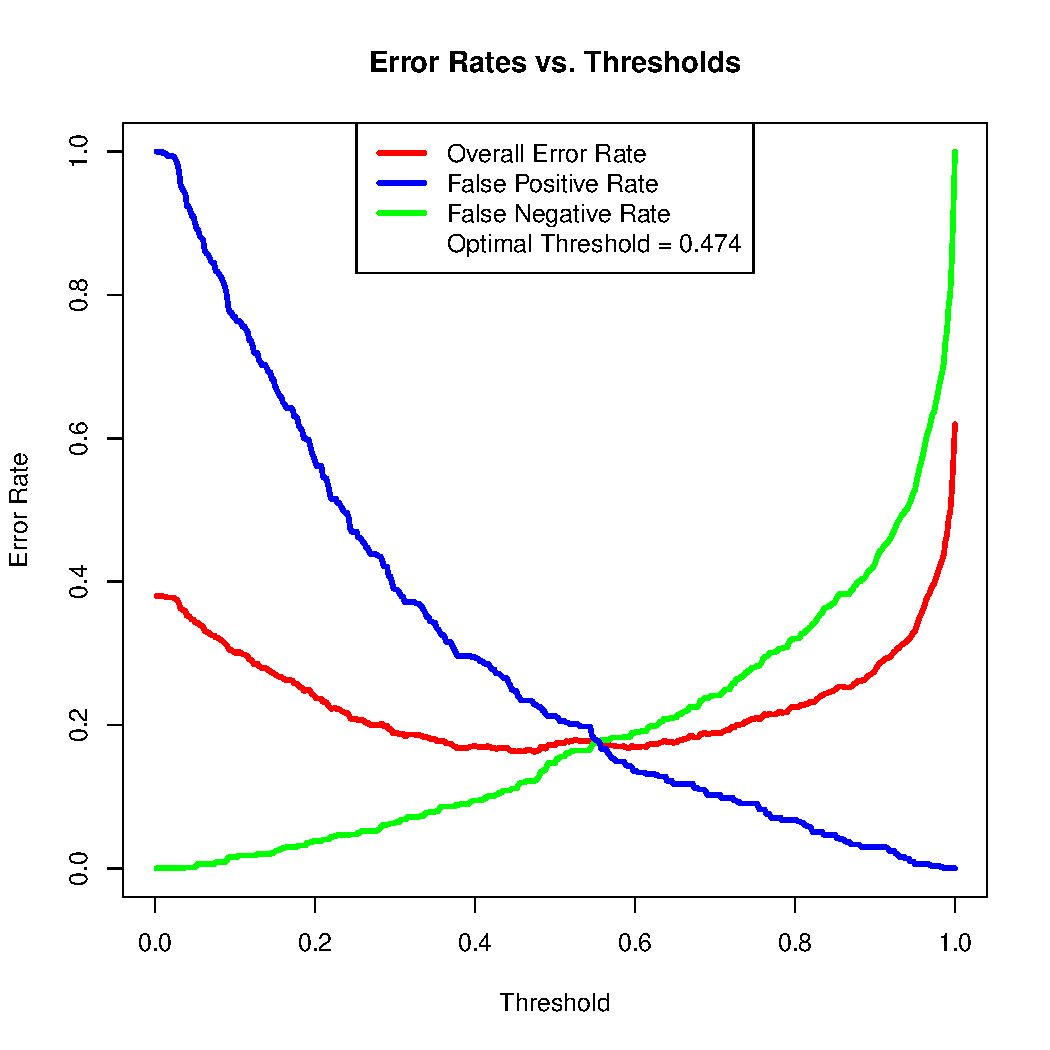
\includegraphics[scale=.4]{../R/out/thresh.pdf}
      \end{figure}\end{center}
    }

    \frame{
      \frametitle{Receiver Operating Characteristics (ROC) Curve}
      \begin{center}\begin{figure}
        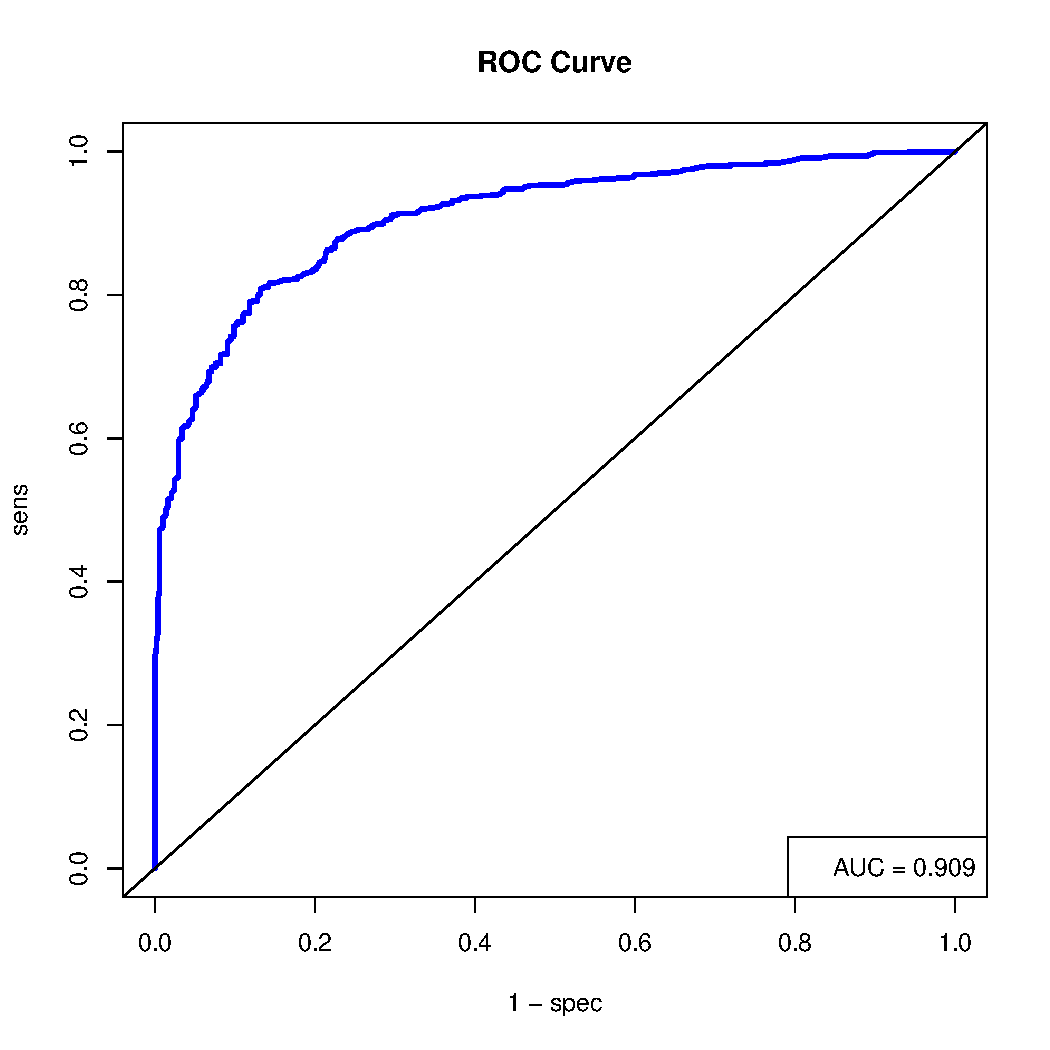
\includegraphics[scale=.4]{../R/out/roc.pdf}
      \end{figure}\end{center}
    }

    \frame{
      \frametitle{Variance Inflation Factors}
      % latex table generated in R 3.0.3 by xtable 1.7-1 package
% Thu Mar 27 07:31:32 2014
\begin{table}[ht]
\centering
\caption{\textbf{VIF Table:}}
\begin{tabular}{rrrr}
  \hline
 %& GVIF & Df & GVIF\verb|^|(1/(2*Df)) \\ 
 & GVIF & Df & GVIF$^{\frac{1}{2Df}}$ \\ 
  \hline
Drugs & 1.12 & 2.00 & 1.03 \\ 
  Belt & 1.24 & 9.00 & 1.01 \\ 
  Speed Related & 1.16 & 2.00 & 1.04 \\ 
  Speed Limit & 1.14 & 1.00 & 1.07 \\ 
  Drink & 1.25 & 1.00 & 1.12 \\ 
  Light & 1.38 & 5.00 & 1.03 \\ 
  Distracted & 1.09 & 2.00 & 1.02 \\ 
  Model year & 1.06 & 1.00 & 1.03 \\ 
   \hline
\end{tabular}
\end{table}

    }
    
    \frame{
      \frametitle{Intuition}
      \begin{center}
        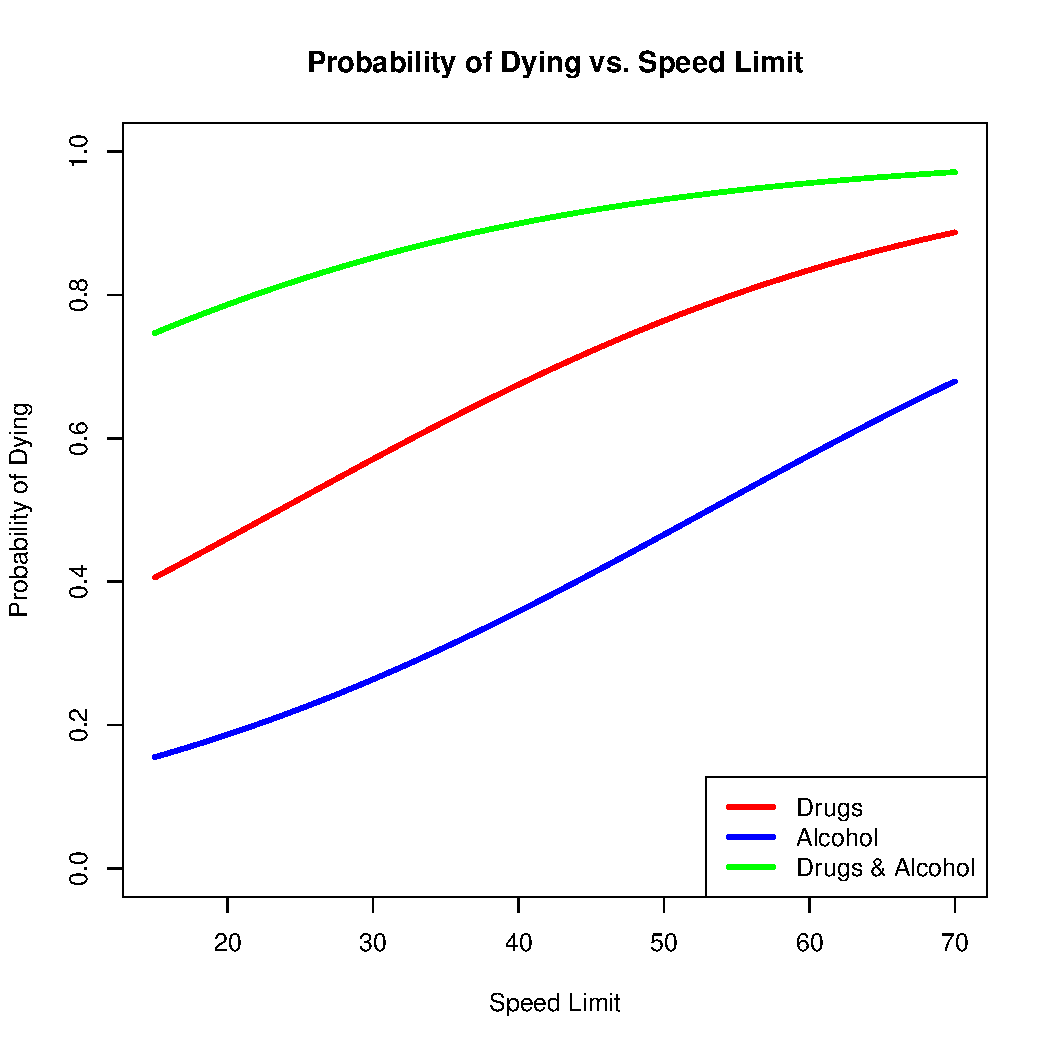
\includegraphics[scale=.4]{../R/out/dd.pdf}
      \end{center}
    }
    
  \section{Conclusions}
    \frame{
      \frametitle{Conclusions}
      \begin{itemize}
        \item Model reduced to 8 covariates using forward selection
        \item AUC = 91\%
        \item VIF $<$ 10
      \end{itemize}
    }

  \section{Future}
    \frame{
      \frametitle{Future}
      \begin{itemize}
        \item Look at other combinations of covariates (interaction)
      \end{itemize}
    }


 
\end{document}
